\section{Results}
\label{sec:results}
We present our joint multi-probe constraints on the cosmological parameters of the flat $\Lambda$CDM parameters in Fig.~\ref{fig:cosmology-params}, showing the marginalised posterior distributions for $\sigma_8$, $\Omega_{\rm m}$ and $h$.   Reporting the best-fit MAP with PJ-HPD values for the two parameters that we are most sensitive to, we find (Blind A)
\eqa{
\sigma_8 &= 0.781^{+0.025}_{-0.019} \\ \nonumber
\Omega_{\rm m} &= 0.31^{+0.011}_{-0.015} \\ \nonumber
S_8 &= 0.791^{+0.020}_{-0.012} \, ,
}
(Blind B)
\eqa{
\sigma_8 &= 0.748^{+0.011}_{-0.030} \\ \nonumber
\Omega_{\rm m} &= 0.293^{+0.024}_{-0.001} \\ \nonumber
S_8 &= 0.740^{+0.014}_{-0.016} \, ,
}
(Blind C)
\eqa{
\sigma_8 &= 0.76^{+0.021}_{-0.023} \\ \nonumber
\Omega_{\rm m} &= 0.306^{+0.011}_{-0.014} \\ \nonumber
S_8 &= 0.769^{+0.018}_{-0.015} \, ,
}
where the BOSS galaxy clustering constraints (GC: shown blue), break the $\sigma_8-\Omega_{\rm m}$ degeneracy in the KiDS-1000 cosmic shear constraints (CS: shown pink), resulting in tight constraints on $\sigma_8$ in the combined $3\times2{\rm pt}$ analysis (shown red).   Our constraints can be compared to the marginalised posterior distributions from Planck (shown green), which we discuss in more detail in Sect.~\ref{sec:planck_comp}.

Tabulated constraints for the full set of cosmological parameters are presented in Appendix~\ref{app:parameter-constraints}, quoting our fiducial MAP with PJ-HPD credible intervals, along with the standard marginal posterior mode with M-HPD credible intervals.   We note that the standard quoted marginal mode constraint on $S_8$ is $\sim 10\%$ tighter than the MAP constraint.  As discussed in \citet{joachimi/etal:inprep}, however, this estimate can be easily misinterpreted, yielding systematically low values of $S_8$ in mock data analyses.   This now known bias, can be seen in Fig.~\ref{fig:S8comp}, which compares the MAP constraints (solid) with the marginal (dashed).  

\begin{figure}
	\begin{center}
		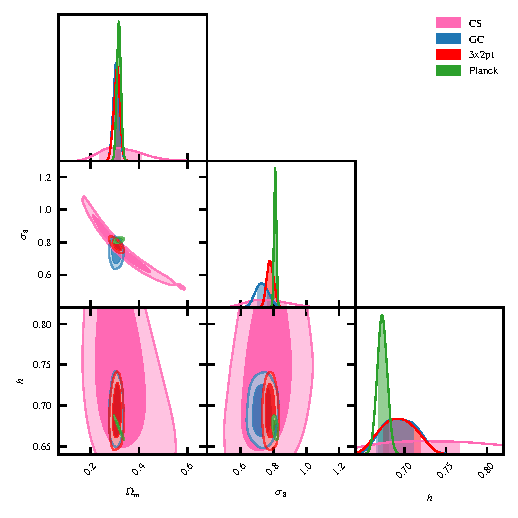
\includegraphics[width=\columnwidth]{Parameter_Plots/cosmology/omegam_sigma8_h_blind_A}
		\caption{Blind A: Multi-probe constraints on the flat $\Lambda$CDM cosmological model, for the matter fluctuation amplitude parameter, $\sigma_8$, the matter density parameter $\Omega_{\rm m}$, and the Hubble parameter, $h$.  The BOSS galaxy clustering constraints (GC: shown blue), can be compared to the KiDS-1000 cosmic shear constraints (CS: shown pink), the combined $3\times2{\rm pt}$ analysis (shown red), and CMB constraints from \citet{planck/etal:2018}.}
		\label{fig:cosmology-params}
	\end{center}
\end{figure}

We find good agreement between the different probe combinations and single probe $S_8$ constraints, demonstrating internal consistency between the different cosmological probes, in Fig.~\ref{fig:S8comp}.  As forecast by \citet{joachimi/etal:inprep}, the addition of the galaxy-galaxy lensing observable adds very little constraining power, with similar results found for the full $3\times2{\rm pt}$ analysis and the combined cosmic shear and clustering analysis.   This is a result of the significant area of BOSS in comparison to KiDS-1000, and the fact that our lack of an accurate non-linear galaxy bias model prohibits the inclusion of large sections of our galaxy-galaxy lensing data vector, shown in Fig.~\ref{fig:Pgk}.     The addition of the galaxy-galaxy lensing does however serve to moderately tighten constraints on the amplitude of the intrinsic alignment model $A_{\rm IA}$. 

\begin{figure}
	\begin{center}
		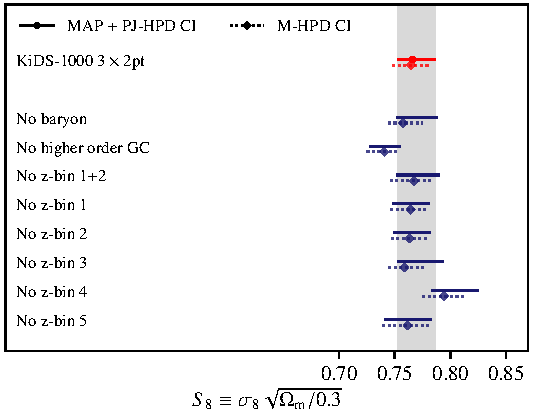
\includegraphics[width=\columnwidth]{Parameter_Plots/systematics/S8_comparison_blindC}
		\caption{Blind C: Constraints on structure growth parameter $S_{8} = \sigma_8 \sqrt{\Omega_{\rm m}/0.3}$ for different probe combinations: $3\times2$pt, cosmic shear with galaxy-galaxy lensing (CS+GGL), and cosmic shear with galaxy clustering (CS+GC), along with the cosmic shear (CS), and galaxy clustering (GC), single probe analyses.   Our fiducial and preferred MAP with PJ-HPD credible interval (solid) can be compared to the standard, but biased, marginal posterior mode with M-HPD credible intervals (dashed).   The lower section of the figure illustrates how our constraints on $S_8$ change when we ignore the impact of baryon feedback (the `No baryon' case), limit the analysis to a linear galaxy bias model (the `No higher order bias' case), and remove individual tomographic bins from our weak lensing observables.    
		\TT{Note that only the 3x2pt chain has the clustering bug fixed, hence the overall offset.}}
		\label{fig:S8comp}
	\end{center}
\end{figure}

The lower section of Fig.~\ref{fig:S8comp} illustrates the results of a series of sensitivity tests, where we explore how our constraints on $S_8$ change when: we ignore the impact of baryon feedback (the `No baryon' case), fixing $A_{\rm baryon}=3.13$, corresponding to the non-linear matter power spectrum for a dark-matter only cosmology; we limit the analysis to a linear galaxy bias model, setting all higher-order bias terms in Eq.(\ref{eq:pgg}), to zero; when we remove individual tomographic bins from our weak lensing observables.    The only outlier in this series of tests is the linear-bias model, which highlights the importance of accurate non-linear galaxy bias modelling in $3\times2$pt analyses.    This series of tests complements the more detailed KiDS-1000 internal consistency analysis of \citet{asgari/etal:inprep}, and is dissected in Appendix~\ref{app:sensitivity}.

Fig.~\ref{fig:cosmology-params-all} displays the marginalised posterior distributions for an extended set of cosmological parameters.   We find that the constraint on galaxy bias,  $b_1$, in each redshift bin (lower two rows), is more than halved with the addition of the weak lensing data.   This constraint does not arise, however, from the sensitivity of the galaxy-galaxy lensing observable to galaxy bias.  Instead, in this analysis, it is a result of the degeneracy breaking in the $\sigma_8-\Omega_{\rm m}$ plane, tightening constraints in $\sigma_8$ which, for galaxy clustering, is fully degenerate with galaxy bias.  The improved constraints on galaxy bias do not, however, fold through to improved constraints on $h$, which the weak lensing data adds very little information to.

For the majority of the cosmological parameters shown in Fig.~\ref{fig:cosmology-params-all}, the constraints are uninformed by our choice of prior.  The three key exceptions are the spectral index, $n_{\rm s}$, the Hubble parameter, $h$, and the baryon feedback amplitude, $A_{\rm baryon}$.  As noted by \citet{troester/etal:2020}, the BOSS galaxy clustering constraints favour a low value for $n_{\rm s}$, where they find $n_{\rm s} = 0.815 \pm 0.085$.  They conclude that this preference is primarily driven by the amplitude of the large scale clustering signal with $s > 100 \, h^{-1}\, {\rm Mpc}$.  As spurious excess power in this regime could plausibly arise from variations in the stellar density impacting the BOSS galaxy selection function \citep{ross/etal:2017}, we chose to impose an informative prior for $n_{\rm s}$, as listed in Table~\ref{tab:priors}.   This prior does not degrade the overall goodness of fit to the galaxy clustering measurements, and is no more informative than the $n_{\rm s}$ priors that are typically used in weak lensing and clustering analyses \citep[see for example][]{sanchez/etal:2017,abbott/etal:2018}.  We do recognise, however, that this choice of prior serves to reduce the BOSS-only error on $\Omega_{\rm m}$ by roughly a third (see Appendix~\ref{app:priors}).   We note that the galaxy clustering preference for low $n_{\rm s}$ also leads to the joint $3\times2{\rm pt}$ constraint favouring the dark-matter only value for the baryon feedback amplitude $A_{\rm baryon}$.   This preference is not significant however, with all values of $A_{\rm baryon}$ within the prior region, compatible at the $<2 \sigma$ level.   BOSS also provides reasonable constraints on $h$, with our $1\sigma$ constraints on $h$ lying within the $h$-prior.   As the marginal probability at the lower prior edge exceeds 20\% of the peak probability, however, we consider this parameter unconstrained by our analysis.

\begin{figure*}
	\begin{center}
		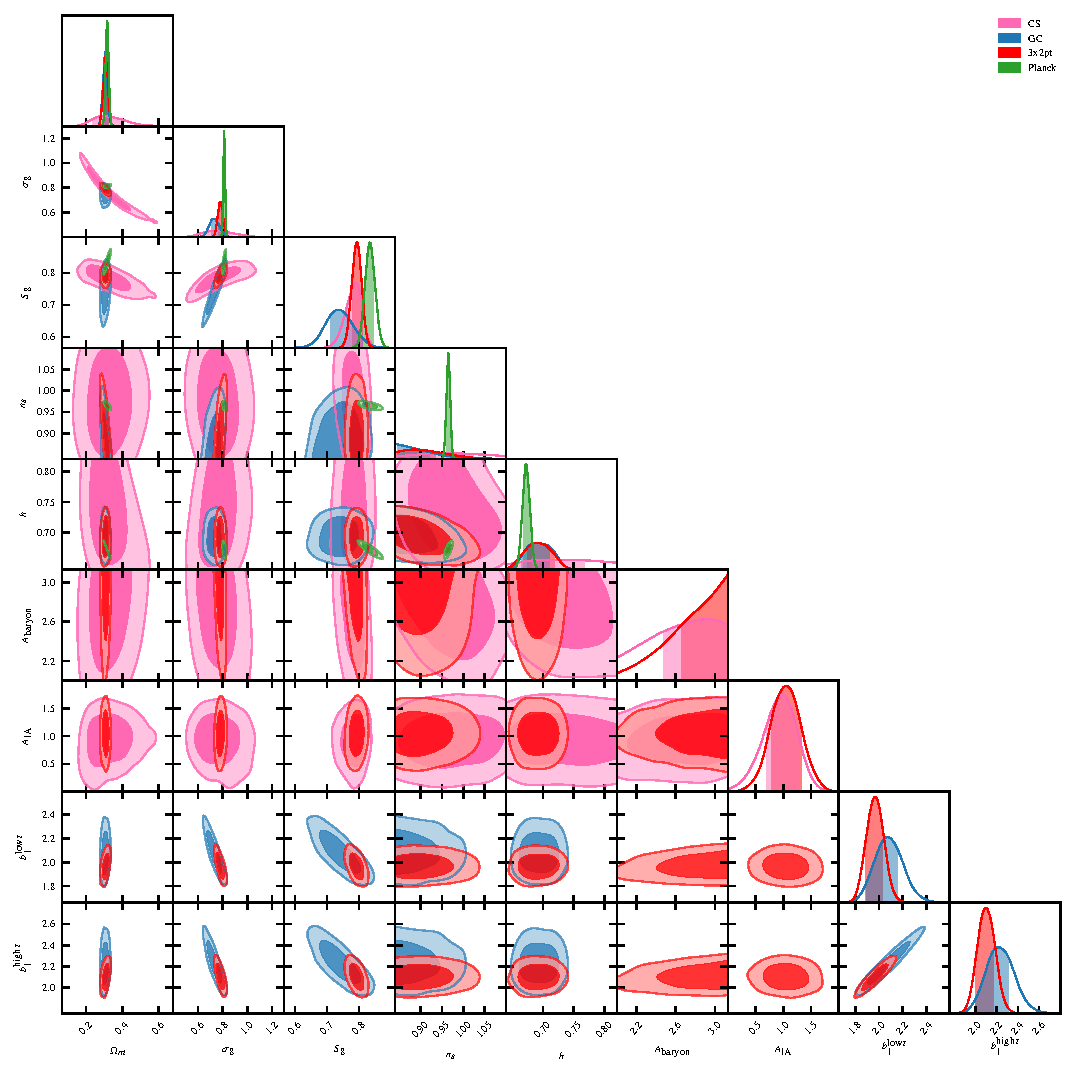
\includegraphics[width=\textwidth]{Parameter_Plots/cosmology/omegam_sigma8_s8_ns_h_a_baryon_a_ia_b1l_b1h_blind_A}
		\caption{Marginalised posterior distributions for an extended set of cosmological parameters covering the matter density parameter $\Omega_{\rm m}$, the matter fluctuation amplitude parameter, $\sigma_8$, the structure growth parameter $S_8$, the spectral index $n_s$, the Hubble parameter, $h$, the baryon feedback amplitude parameter, $A_{\rm baryon}$, the intrinsic alignment amplitude, $A_{\rm IA}$, and the linear bias parameters for the low and high BOSS redshift bins, $b_1$.   The KiDS-1000 cosmic shear results (CS, pink), can be compared to the BOSS galaxy clustering results (GC, blue), and their combinations CS+GC (purple), and the full $3\times2$pt, including BOSS and 2dFLenS galaxy-galaxy lensing (red).   For parameters constrained by the CMB, we also include constraints from \citet{planck/etal:2018} (green).}
		\label{fig:cosmology-params-all}
	\end{center}
\end{figure*}

Table~\ref{tab:goodness-of-fit} records the goodness of fit for each component in our $3\times2$pt analysis.  The effective number of degrees of freedom (DoF) are calculated using the estimator described in section 6.3 of \citet{joachimi/etal:inprep}.   The goodness of fit in all cases is acceptable, but only just.    We are unconcerned by these results, however, given the cosmic shear analysis of \citet{asgari/etal:inprep}, where a different choice in the cosmic shear two-point statistic results in an excellent goodness of fit, with no significant changes in the inferred cosmological parameters.    As such, we could be subject to an unlucky noise fluctuation that particularly impacts the band power estimator in Eq.(\ref{eq:cl_cosmicshear}.  Cautiously inspecting Fig.~\ref{fig:Pkk}, as `$\chi$-by-eye' is particularly dangerous with correlated data points, we nevertheless note a handful of outlying points, for example the low$\ell$-scales in the fifth tomographic bin.   We also note that \citet{giblin/etal:inprep} document a significant but low-level PSF residual systematic in the KiDS-1000 fourth and fifth tomographic bins that was shown to reduce the overall goodness of fit in a cosmic shear analysis, but not bias the recovered cosmological parameters \citep[see also the discussion in][]{amara/refregier:2008}.  Future work to remove these low-level residual distortions are therefore expected to improve the goodness of fit further.

\begin{table}
	\begin{center}
		\caption{The goodness of fit of the MAP cosmological model for each of the single and joint probe combinations with cosmic shear (CS), galaxy clustering (GC) and galaxy-galaxy lensing (GGL).   We list the $\chi^2$ value for each MAP model, the effective number of degrees of freedom (DoF) and the corresponding $p$-value which describes the probability of producing measurements that are more extreme than the data, assuming the MAP model is correct.   For reference, $p > 0.001$ corresponds to $<3\sigma$ events.}
		\label{tab:goodness-of-fit}
\begin{tabular}{lrcl}
    \toprule
    Probe             & $\chi^2$       & DoF       & $p$-value   \\
    \midrule
	CS               & $< 156.3$ & $120-4.5$ & 0.007 \\
	GC               & $< 169.5$ & $168-13$ & 0.202 \\
	CS+GGL           & $187.0$ & $142-7$ & 0.002 \\
	$3\times2$pt            & $367.8$ & $310-20$ & 0.001 \\

    \bottomrule
\end{tabular}
	\end{center}
\end{table}


\subsection{Comparison with Planck}
\label{sec:planck_comp}
This section we will write post-blinding, as until we know which blind it is, it is hard to write.   The short version is A: no tension,  B: oodles of tension,  C: hum.....



